\documentclass[12pt]{article}
\usepackage{amsmath}
\usepackage{amssymb}
\usepackage[letterpaper,top=1.35in,bottom=0.75in,left=0.75in,right=0.75in,centering]{geometry}
\usepackage{fancyhdr}
\usepackage{enumerate}
\usepackage{lastpage}
\usepackage{multicol}
\usepackage{graphicx}
\usepackage{vwcol}
\reversemarginpar

\pagestyle{fancy}
\cfoot{Page \thepage \ of \pageref{LastPage}}\rfoot{{\bf Total Points: 30}}
\lhead{\hspace*{2.2in}\underline{MATH 1560: Test 6}}

\newcommand{\points}[1]{\marginpar{\hspace{24pt}[#1]}}
\newcommand{\skipline}{\vspace{12pt}}
\renewcommand{\headrulewidth}{0in}
\headheight 20pt

\newcommand{\di}{\displaystyle}
\newcommand{\abs}[1]{\lvert #1\rvert}
\newcommand{\R}{\mathbb{R}}
\newcommand{\C}{\mathbb{C}}
\renewcommand{\P}{\mathcal{P}}
\DeclareMathOperator{\nul}{null}
\DeclareMathOperator{\range}{range}
\DeclareMathOperator{\spn}{span}
\newcommand{\len}[1]{\lVert #1\rVert}
\newcommand{\Q}{\mathbb{Q}}
\newcommand{\N}{\mathbb{N}}
\renewcommand{\L}{\mathcal{L}}
\newcommand{\dotp}{\boldsymbol{\cdot}}
\newenvironment{amatrix}[1]{%
  \left[\begin{array}{@{}*{#1}{c}|c@{}}
}{%
  \end{array}\right]
}
\newcommand{\bam}{\begin{amatrix}}
\newcommand{\eam}{\end{amatrix}}
\newcommand{\bbm}{\begin{bmatrix}}
\newcommand{\ebm}{\end{bmatrix}}

\begin{document}
\begin{center}
{\bf MATH 1560 - Test \#6 Solutions}\\
Examiner: Sean Fitzpatrick
\end{center}

 \begin{enumerate}
 \item  Compute the following antiderivatives:
 \begin{enumerate}
 \item The antiderivative $F$ of $f(x) = 2x+\sec^2(x)$ such that $F(0)=4$. \points{3}
 
\medskip

We have $F(x)=x^2+\tan(x)+C$ for some $C$. Since $F(0)=4$,
\[
4 = F(0) = 0^2+\tan(0)+C = C
\]
so $C=4$ and $F(x) = x^2+\tan(x)+4$.

\bigskip
 
 \item  \points{3} \begin{align*}
 \int (3x^2+2\sqrt{x}-5)\,dx &= \int(3x^2+2x^{1/2}-5)\,dx\\
&= 3\left(\frac{1}{3}x^3\right)+2\left(\frac{2}{3}x^{3/2}\right)-5x+C\\
& = x^3+\frac{4}{3}x^{3/2}-5x+C
 \end{align*} 
 
\medskip





 
 \item $\di \int \left(\cos(x)-\frac{1}{\sqrt{1-x^2}}\right)\,dx = \sin(x)-\arcsin(x)+C$ \points{3}
 
 \bigskip
 
 \item $\di \int x^3 e^{x^4+2}\,dx$ \points{3}
 
 \medskip
 
 Letting $u=x^4+2$, we have $du = 4x^3\,dx$, so $\frac{1}{4}\,du = x^3\,dx$ and
 \[
 \int x^3 e^{x^4+2}\,dx = \int e^u\cdot \frac{1}{4}\,du = \frac{1}{4}e^u+C = \frac{1}{4}e^{x^4+2}+C.
 \]
 \end{enumerate}
 \newpage
 
 \item Use Part I of the Fundamental Theorem of Calculus to compute the derivatives of the following functions:
 \begin{enumerate}
 \item $\di F(x) = \int_2^x \sin(t^2+3t)\,dt$ \points{2}
 
 \medskip
 
 By direct application of FTC I, since our integrand is $f(t)=\sin(t^2+3t)$, we have
 \[
 F'(x) = f(x) = \sin(x^2+3x).
 \]
 
 \medskip
 
 \item $\di G(x) = \int_x^{x^2}\sqrt{t^4+1}\,dt$ \points{3}
 
 First, we re-write $G(x)$ using properties of integrals:
 
 \[
 G(x) = \int_x^0 \sqrt{t^4+1}\,dt + \int_0^{x^2}\sqrt{t^4+1}\,dt = -\int_0^x\sqrt{t^4+1}\,dt + \int_0^{x^2}\sqrt{t^4+1}\,dt.
 \]
 
 For the second integral, we use the fact that combining the Chain Rule with FTC I gives us
 \[
 \frac{d}{dx}\int_a^{g(x)}f(t)\,dt = f(g(x))g'(x).
 \]
 Thus, we find
 \[
 G'(x) = -\sqrt{x^4+1}+\sqrt{(x^2)^4+1}(2x) = 2x\sqrt{x^8+1}-\sqrt{x^4+1}.
 \]
 
 \bigskip
 
  \end{enumerate}
 \item Use Part II of the Fundamental Theorem of Calculus to evaluate the following definite integrals:
 \begin{enumerate}
 \item \points{3}\begin{align*}
   \int_0^1\left(3x^2-2x+4\right)\,dx & = \left.x^3-x^2+4x\right|_0^1\\
   & = 1^3-1^2+4(1)-(0^3-0^2+4(0)) = 4.
 \end{align*}

 \bigskip
 
  
 \item $\di \int_0^{\pi/2}\cos(x)\sin^3(x)\,dx$ \points{4}
 
 \medskip
 
 Letting $u=\sin(x)$, we have $du = \cos(x)\,dx$, and when $x=0$, $u=\sin(0)=0$, and when $x=\pi/2$, $u=\sin(0)=1$. Thus,
 
 \[
 \int_0^{\pi/2}\cos(x)\sin^3(x)\,dx = \int_0^1 u^3\,du = \left.\frac{1}{4}u^4\right|_0^1 = \frac{1}{4}.
 \]
 \end{enumerate}
 \newpage
 
 Extra group questions!
 
 \item Evaluate the integral $\di \int_0^2 \abs{2x-2}\,dx$. \points{3}
 
\noindent Suggestion: either use properties of integrals to simplify, or sketch the graph and evaluate by interpreting the result as an area.

\medskip

Since 
\[
\abs{2x-2} = \begin{cases}2x-2 & \text{ if } 2x-2\geq 0\\ -(2x-2) & \text{ if } 2x-2<0\end{cases} = \begin{cases} 2x-2 & \text{ if } x\geq 1\\ 2-2x & \text{ if } x<1,\end{cases}
\]
we have
\begin{align*}
\int_0^2 \abs{2x-2}\,dx & = \int_0^1\abs{2x-2}\,dx+\int_1^2\abs{2x-2}\,dx\\
& = \int_0^1 (2-2x)\,dx + \int_1^2 (2x-2)\,dx\\
& = \left(\left.2x-x^2\right|_0^1\right) + \left(\left.x^2-2x\right|_1^2\right)\\
& = (2(1)-1^2-(0-0))+ ( 2^2-2(2) - (1^2-2(1)))\\
& = 1+1 = 2.
\end{align*}

\begin{multicols}{2}
Alternatively, from the sketch of the graph (shown on the right), we see that the area consists of the area of two triangles, each with base 1 and height 2. Thus, the integral is equal to the area
\[
A = \frac{1}{2}(1)(2)+\frac{1}{2}(1)(2) = 2.
\]
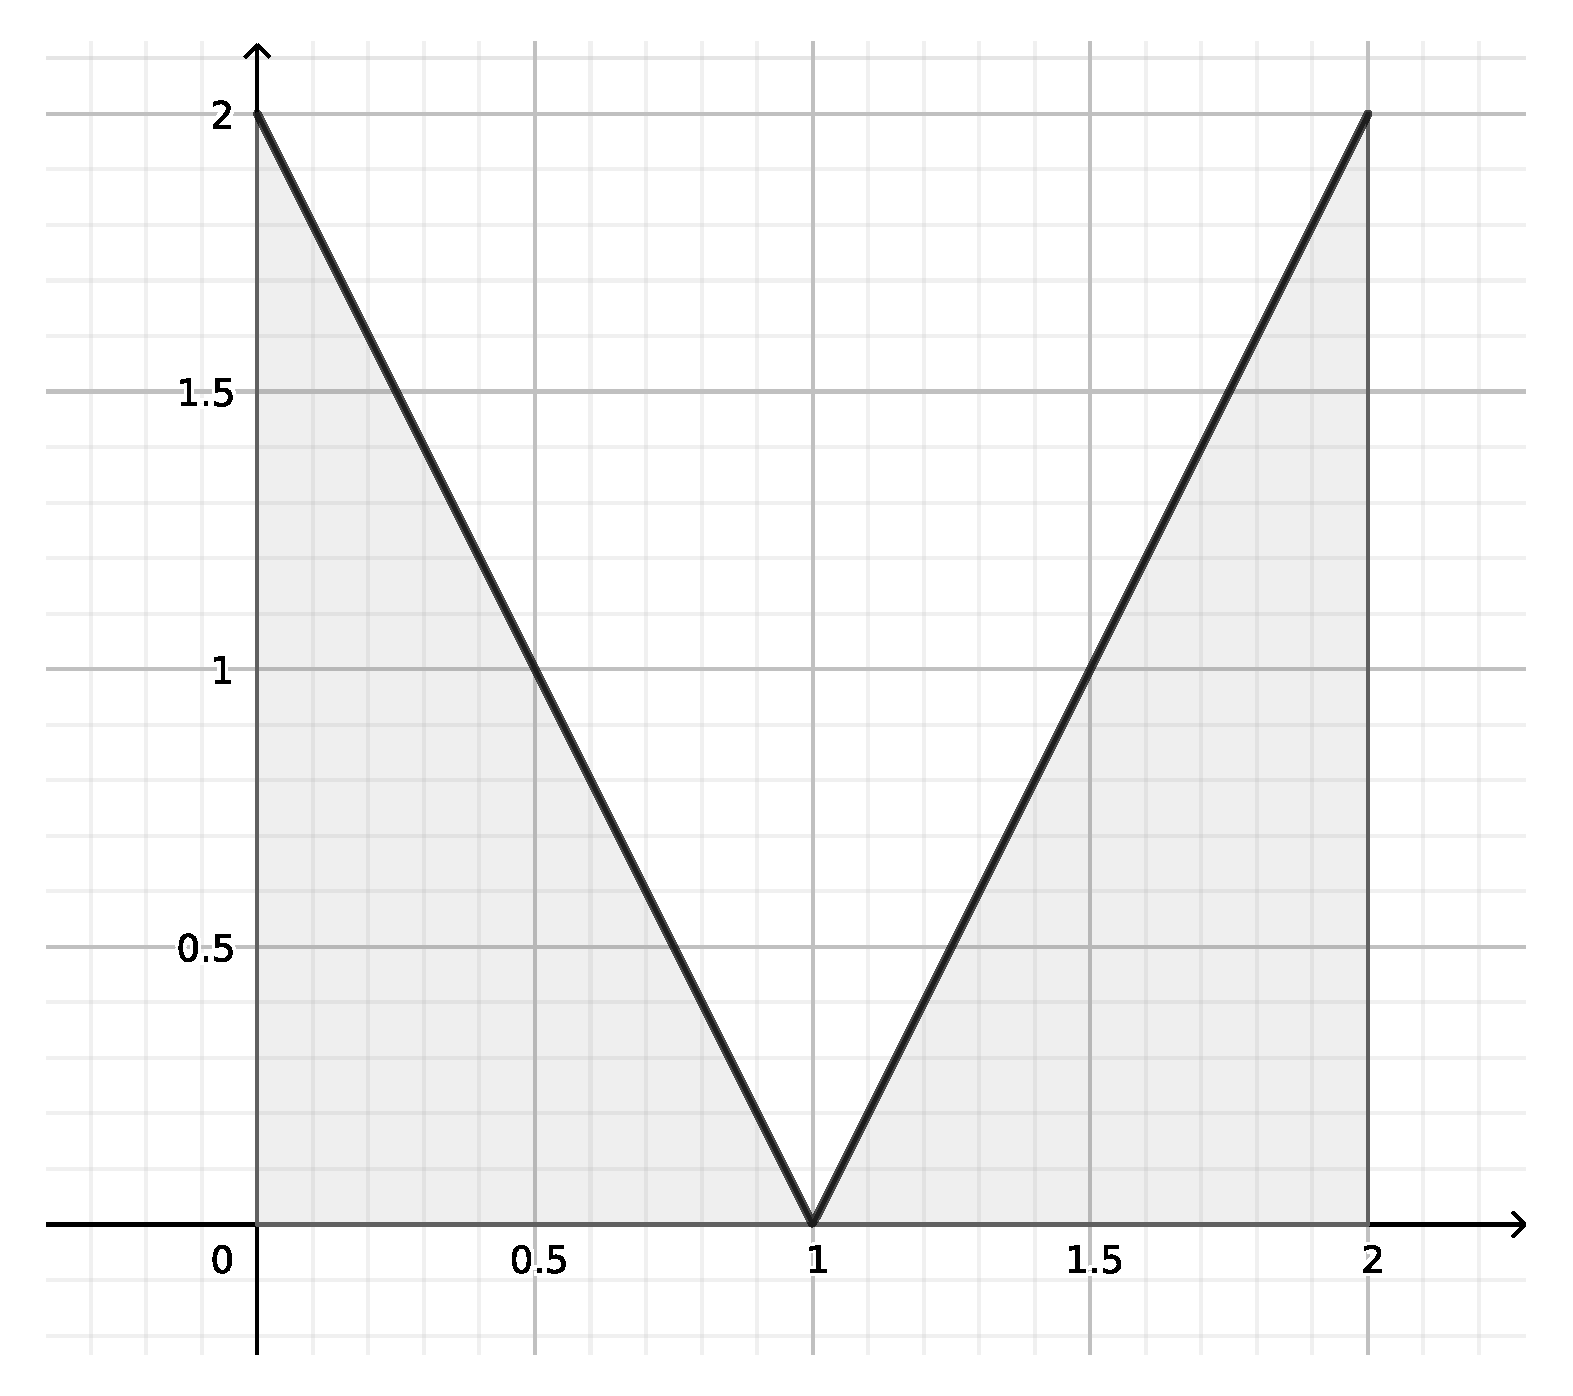
\includegraphics[width=\columnwidth]{TT6-fig1}
\end{multicols}

\newpage

 \item Find the area between the curves $y= 2-x^2$ and $y=x^2$ for $0\leq x\leq 3$. \points{3}
 


First, we note that if $2-x^2=x^2$, then $2=2x^2$, so the curves intersect when $x^2=1$, or $x=\pm 1$. For $0\leq x\leq 3$, this gives us the point of intersection when $x=1$.

We note that for $0\leq x\leq 1$, $2-x^2\geq x^2$, while for $1\leq x\leq 3$, $x^2\geq 2-x^2$. Our area is therefore
\begin{align*}
A = \int_0^3\abs{(2-x^2)-x^2}\,dx &= \int_0^1 (2-2x^2)\,dx + \int_1^3 (2x^2-2)\,dx\\
&=\left(\left. 2x-\frac{2}{3}x^3\right|_0^1\right) +\left(\left.\frac{2}{3}x^3-2x\right|_1^3\right)\\
&=\left(2(1)-\frac{2}{3}(1)-(0-0)\right)+\left(\frac{2}{3}(27)-2(3)-(\frac{2}{3}(1)-2(1)\right)\\
&=2-\frac{2}{3}+18-6-\frac{2}{3}+2 = 16-\frac{4}{3} = \frac{44}{3}.
\end{align*}
\begin{center}
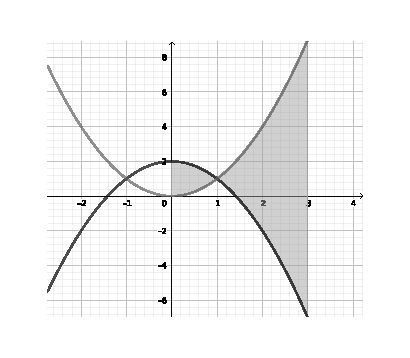
\includegraphics[width=4in]{TT6-fig2}
\end{center}

\end{enumerate}
\end{document}